\documentclass[a4paper,12pt]{article}

% Packages
\usepackage[utf8]{inputenc} % Encoding
\usepackage[T1]{fontenc}  % Font encoding
\usepackage[colorlinks=true,linkcolor=blue,urlcolor=blue,citecolor=blue]{hyperref}     % Hyperlinks
\usepackage{geometry}     % Page layout
\usepackage{listings}     % Code listings
\usepackage{xcolor}       % Colors for code
\usepackage{tcolorbox} % Add this to your preamble


% Page layout
\geometry{margin=1in}

% Functions
\tcbset{
    attentionbox/.style={
        colback=red!5, % Background color
        colframe=red!75!black, % Border color
        coltitle=black, % Title color
        boxrule=0.8mm, % Thickness of the border
        left=2mm, % Left padding
        before skip=5mm, % Space before the box
        after skip=5mm, % Space after the box
        sharp corners, % Sharp corners for the box
        fonttitle=\bfseries, % Bold title font
        attach boxed title to top left={yshift=-2mm,xshift=2mm}, % Title position
        boxed title style={
            size=small,
            colback=red!50,
            colframe=red!75!black,
            sharp corners,
        },
    }
}

% % Code formatting
\lstset{
    language=Python,
    basicstyle=\ttfamily\fontsize{9}{10}\selectfont,
    breaklines=true,
    frame=single,
    keywordstyle=\color{blue},
    commentstyle=\color{green!70!black},
    stringstyle=\color{red},
    showstringspaces=false,
    numbers=left,
    numberstyle=\tiny\color{gray},
    stepnumber=1,
    numbersep=10pt,
    xleftmargin=5mm,
}

% Metadata
\title{Developer Guide for Project \texttt{HDF5\_BLS}}
\author{Pierre Bouvet}
\date{\today}

\begin{document}

\maketitle


\begin{tcolorbox}[title=Why are you here?]
    \begin{itemize}
        \item \hyperref[sec:load_data]{I want to import my data to the HDF5 file format}
        \item \hyperref[sec:treatment]{I want to extract information from my data }
    \end{itemize}
\end{tcolorbox}

\section{Load data} \label{sec:load_data}

    \begin{tcolorbox}
        Are you using a format that is already supported by the \texttt{HDF5\_BLS} package?
        \begin{itemize}
            \item \hyperref[subsec:load_data.user_specific]{Yes but it doesn't work with my data.}
            \item \hyperref[subsec:load_data.improvement]{Yes but I would like to improve the code.}
            \item \hyperref[subsec:load_data.new_format]{No, I would like to add support for my data.}
        \end{itemize}
    \end{tcolorbox}

    \subsection{Adding a user-specific function to an already supported format} \label{subsec:load_data.user_specific}

        \begin{tcolorbox}
            You are in the situation where you are using a format that is already supported by the \texttt{HDF5\_BLS} package (for example ".dat") but that doesn't work with your data.
        \end{tcolorbox}

        Here are the steps to follow:
        \begin{enumerate}
            \item Locate the python file that handles your data format in the \texttt{load\_formats} folder of the \texttt{HDF5\_BLS} package. The name of the file should correspond to the name of the format you are using (for example "load\_dat.py" if you are using ".dat" files).
            \item Add the function that will load your data to the file. The function should have the following signature:
\begin{lstlisting}
def load_dat_Wien(filepath, parameters = None):
\end{lstlisting}
            In the case where you don't need to load the data with parameters, the function should have the following signature:
\begin{lstlisting}
def load_dat_Wien(filepath):
\end{lstlisting}
            \item Write the code that will load your data. Your function should retunr a dictionnary with at least two keys: "Data" and "Attributes". The "Data" key should contain the data you are loading and the "Attributes" key should contain the attributes of the file. You can also add abscissa to your data if you want to, in that case, add the key "Abscissa\_\textsl{name}" where \textsl{name} is the name you want to give to the abscissa (for example "Abscissa\_Time").
            \item Go to the \texttt{load\_data.py} file in the \texttt{HDF5\_BLS} package and locate the function dedicated to the format you are using (for example "load\_dat\_file" if you are using ".dat" files)
            \item Make sure that you are importing the function you just created:
\begin{lstlisting}
from HDF5_BLS.load_formats.load_dat import load_dat_Wien
\end{lstlisting}
            \item Then, define an identifier for your function (for example "Wien") and either create or add your identifier to the if-else statement. Don't forget to add your identifier to the "creator\_list" list in the "else" statement:
\begin{lstlisting}
if creator == "GHOST": return load_dat_GHOST(filepath)
...
elif creator == "Wien": return load_dat_Wien(filepath)
else:
    creator_list = ["GHOST", "TimeDomain", "Wien"]
    raise LoadError_creator(f"Unsupported creator {creator}, accepted values are: {', '.join(creator_list)}", creator_list)
\end{lstlisting}
            \item Add a test to the function in the "tests/load\_data\_test.py" file with a test file placed in the "tests/test\_data" folder. This test is important as they are run automatically when the package is pushed to GitHub (ie: it makes my life easier ^^). 
            \item You can now use your data format with the \texttt{HDF5\_BLS} package, and in particular, the GUI. You are invited to push your code to GitHub and create a pull request to the main repository :)
        \end{enumerate}

    \subsection{Improving an already supported function} \label{subsec:load_data.improvement}
        \begin{tcolorbox}
            You are in the situation where you want to improve a load function of the \texttt{HDF5\_BLS} package (for example ".dat").
        \end{tcolorbox}

        Here are the steps to follow:
        \begin{enumerate}
            \item Locate the python file that handles your data format in the \texttt{load\_formats} folder of the \texttt{HDF5\_BLS} package. The name of the file should correspond to the name of the format you are using (for example "load\_dat.py" if you are using ".dat" files).
            \item Locate the function that loads your data. The function should have a name similar to (might not have parameters):
\begin{lstlisting}
def load_dat_Wien(filepath, parameters = None):
\end{lstlisting}
            \item Update the code. One good measure is to duplicate the function and comment one of the two versions. Then, write your code and run the tests. If the tests fail, you can always go back to the previous version. Note that if the test fails, the code cannot be pushed to GitHub.
            \item If everything is sound, you can now use your new function with the \texttt{HDF5\_BLS} package. You are invited to push your code to GitHub and create a pull request to the main repository :)
            \item Note: If you want to improve the loading of the data to the hdf5 file (chunking for example), please contact the maintainer directly.
        \end{enumerate}

    \subsection{Adding a user-specific function to an already supported format} \label{subsec:load_data.new_format}

        \begin{tcolorbox}
            You are in the situation where you are using a new format that is not supported by the \texttt{HDF5\_BLS} package.
        \end{tcolorbox}

        Here are the steps to follow:
        \begin{enumerate}
            \item Navigate to the \texttt{load\_formats} folder of the \texttt{HDF5\_BLS} package. 
            \item Create a new python file with the name of the format you are using (for example "load\_unicorn.py" if you are using ".unicorn" files).
            \item Add the function that will load your data to the file. The function should have the following signature:
\begin{lstlisting}
def load_unicorn_Wien(filepath, parameters = None):
\end{lstlisting}
            In the case where you don't need to load the data with parameters, the function should have the following signature:
\begin{lstlisting}
def load_dat_Wien(filepath):
\end{lstlisting}
            \item Write the code that will load your data. Your function should retunr a dictionnary with at least two keys: "Data" and "Attributes". The "Data" key should contain the data you are loading and the "Attributes" key should contain the attributes of the file. You can also add abscissa to your data if you want to, in that case, add the key "Abscissa\_\textsl{name}" where \textsl{name} is the name you want to give to the abscissa (for example "Abscissa\_Time").
            \item Go to the \texttt{load\_data.py} file in the \texttt{HDF5\_BLS} package and create the function dedicated to the format you are using (for example "load\_unicorn\_file" if you are using ".unicorn" files)
            \item Make sure that you are importing the function you just created:
\begin{lstlisting}
from HDF5_BLS.load_formats.load_unicorn import load_unicorn_Wien
\end{lstlisting}
            \item Add a test to the function in the "tests/load\_data\_test.py" file with a test file placed in the "tests/test\_data" folder. This test is important as they are run automatically when the package is pushed to GitHub (ie: it makes my life easier ^^). 
            \item You can now use your data format with the \texttt{HDF5\_BLS} package, and in particular, the GUI. You are invited to push your code to GitHub and create a pull request to the main repository :)
        \end{enumerate}

\section{Treat data} \label{sec:treatment}

    \begin{tcolorbox}
        What is the format of your data?
        \begin{itemize}
            \item \hyperref[subsec:treatment.toPSD]{I just have raw data coming from the spectrometer}
            \item \hyperref[subsec:treatment.toInfo]{I have a Spectral Power Density together with a frequnecy vector}
            \item \hyperref[subsec:treatment.new]{I want to define a new treatment function}
        \end{itemize}
    \end{tcolorbox}

    \subsection{Treat data to obtain a Power Spectral Density and a frequency vector} \label{subsec:treatment.toPSD}
        \begin{tcolorbox}
            To do
        \end{tcolorbox}

    \subsection{Treat data to extract information from a Power Spectral Density} \label{subsec:treatment.toInfo}

        Here are the steps to follow for the GUI compatibility:
        \begin{enumerate}
            \item If "type" is the type of your spectrometer, add the function "treat\_type" in the "HDF5\_BLS\_GUI/treat\_ui.py" file. For example if your spectrometer type is "Unicorn", add the following function:
\begin{lstlisting}
def treat_unicorn
\end{lstlisting}
            \item Add the following parameters to your function:
            \begin{itemize}
                \item parent: the parent GUI window
                \item wrp: the wrapper associated to the main h5 file
                \item path: the path to the data we want to treat in the form "Data/Data/..."
            \end{itemize}
\begin{lstlisting}
def treat_unicorn(parent, wrp, path):
\end{lstlisting}
            \item Define your function. You can find an example of how it was done for the "TFP" treatment in the \hyperref[subsec:example_treatment.TFP]{appendix}.
        \end{enumerate}
    
    \subsection{Adding a new treatment function} \label{subsec:treatment.new}


\section*{Contact}
For questions or suggestions, please contact the maintainer at:

\begin{center}
    \href{mailto:pierre.bouvet@meduniwien.ac.at}{pierre.bouvet@meduniwien.ac.at}.
\end{center}





\appendix 







\section{Examples of treatment pipelines}

    \subsection{Treatment of a TFP spectrometer} \label{subsec:example_treatment.TFP}

        \begin{tcolorbox}
            We here present the code that was used to treat the data obtained from a TFP spectrometer. This code is meant to be used as an example of how to write a treatment function for the GUI compatibility. 
        \end{tcolorbox}

        \begin{enumerate}
            \item We first extract all the PSDs and frequency arrays that are child of the element that has been selected. To do that, we need to go through all the higher layers of our wrapper until our data is found. This is done using the following code:
\begin{lstlisting}
def get_paths_childs(wrp, path = "", frequency = None):
    child, freq = [], []
    if "Frequency" in wrp.data.keys():
        frequency = path+"/Frequency"
    for e in wrp.data.keys():
        if isinstance(wrp.data[e], wrapper.Wrapper):
            ce, fe = get_paths_childs(wrp.data[e], path+"/"+e, frequency=frequency)
            child += ce
            freq += fe
        else:
            if e == "Power Spectral Density":
                freq.append(frequency)
                child.append(path+"/"+e)
    return child, freq
        
# Get the selected data wrapper and frequency array
wrp_temp = wrp
path_loc = path.split("/")[1:]
if "Frequency" in wrp.data.keys(): frequency = wrp.data["Frequency"]
else: frequency = None
for e in path_loc: 
    if "Frequency" in wrp_temp.data[e].data.keys(): 
        frequency = wrp_temp.data[e].data["Frequency"]
    if isinstance(wrp_temp.data[e], wrapper.Wrapper): 
        wrp_temp = wrp_temp.data[e]

childs, frequency = get_paths_childs(wrp_temp, path)
\end{lstlisting}
        \item From there we have a choice to make: either we treat each PSD individually or all at once, from some globally defined parameters. We therefore need to ask the user if he wants to treat all of them with the same parameters or each one individually. This is done using the following code:
\begin{lstlisting}
# Display a dialog box to ask the user if he wants to treat all of them with the same parameters or each one individually
msgBox = qtw.QMessageBox()        
msgBox.setText(f"There are {len(childs)} PSD in the selected data. Do you want to treat all of them at once?")
msgBox.setStandardButtons(qtw.QMessageBox.Yes | qtw.QMessageBox.No | qtw.QMessageBox.Cancel)
msgBox.setDefaultButton(qtw.QMessageBox.Yes)
ret = msgBox.exec()
if ret == qtw.QMessageBox.Yes: 
    # Treat all PSD at once
elif ret == qtw.QMessageBox.No:
    # Treat each PSD individually
\end{lstlisting}
        \item In both cases, we will want to open a window to enter the parameters of the treatment. In the first case, where all the spectra are treated at once, we open the window with all the spectra as parameters. In the second case, where each spectrum is treated individually, we will have a "for" loop to open the window for each spectrum. This is done using the following code:
\begin{lstlisting}
from ParameterCurve.main import TFP_treat

if ret == qtw.QMessageBox.Yes: 
    dialog = TFP_treat(parent = parent, wrp_base = wrp, path_base = path, path_curves = childs, path_frequency = frequency)
    if dialog.exec_() == qtw.QDialog.Accepted:
        # Store all the treated values
elif ret == qtw.QMessageBox.No:
    for c,f in zip(childs, frequency):
        dialog = TFP_treat(parent = parent, wrp_base = wrp, path_base = path, path_curves = childs, path_frequency = frequency)
        if dialog.exec_() == qtw.QDialog.Accepted:
            # Store the treated values
\end{lstlisting}
        Note that here we are importing another GUI window from the \texttt{ParameterCurve} package. The definition of this GUI window is therefore the next step. Let's now look into this \texttt{TFP\_treat} class.
        \item Opening the "HDF5\_BLS\_GUI/ParameterCurve/main.py" file, we define the \texttt{TFP\_treat} class as a daughter of the \texttt{ParameterCurve} class, which is a GUI window with 4 distinct elements:
        \begin{itemize}
            \item A combobox to select the curves to plot at the top left of the window.
            \item A combobox to select the function to apply at the top right of the window.
            \item A graph frame to display the curves at the bottom left of the window.
            \item A frame to display the parameters of the treatment at the bottom right of the window, together with buttons to apply the treatment and to close the window.
        \end{itemize}:
\begin{lstlisting}
class TFP_treat(ParameterCurve):
    def __init__(self, parent=None, wrp_base = None, path_base = None, path_curves = None, path_frequency = None):
        super().__init__(parent, wrp_base.get_child(path_base))
\end{lstlisting}
        This initializes the \texttt{ParameterCurve} class with the wrapper corresponding to all the curves we are going to treat. Giving the class the path of the selected curves displays them by default in the combobox.
        Here is an image of a raw ParameterCurve window after this simple initialization:
        \begin{center}
            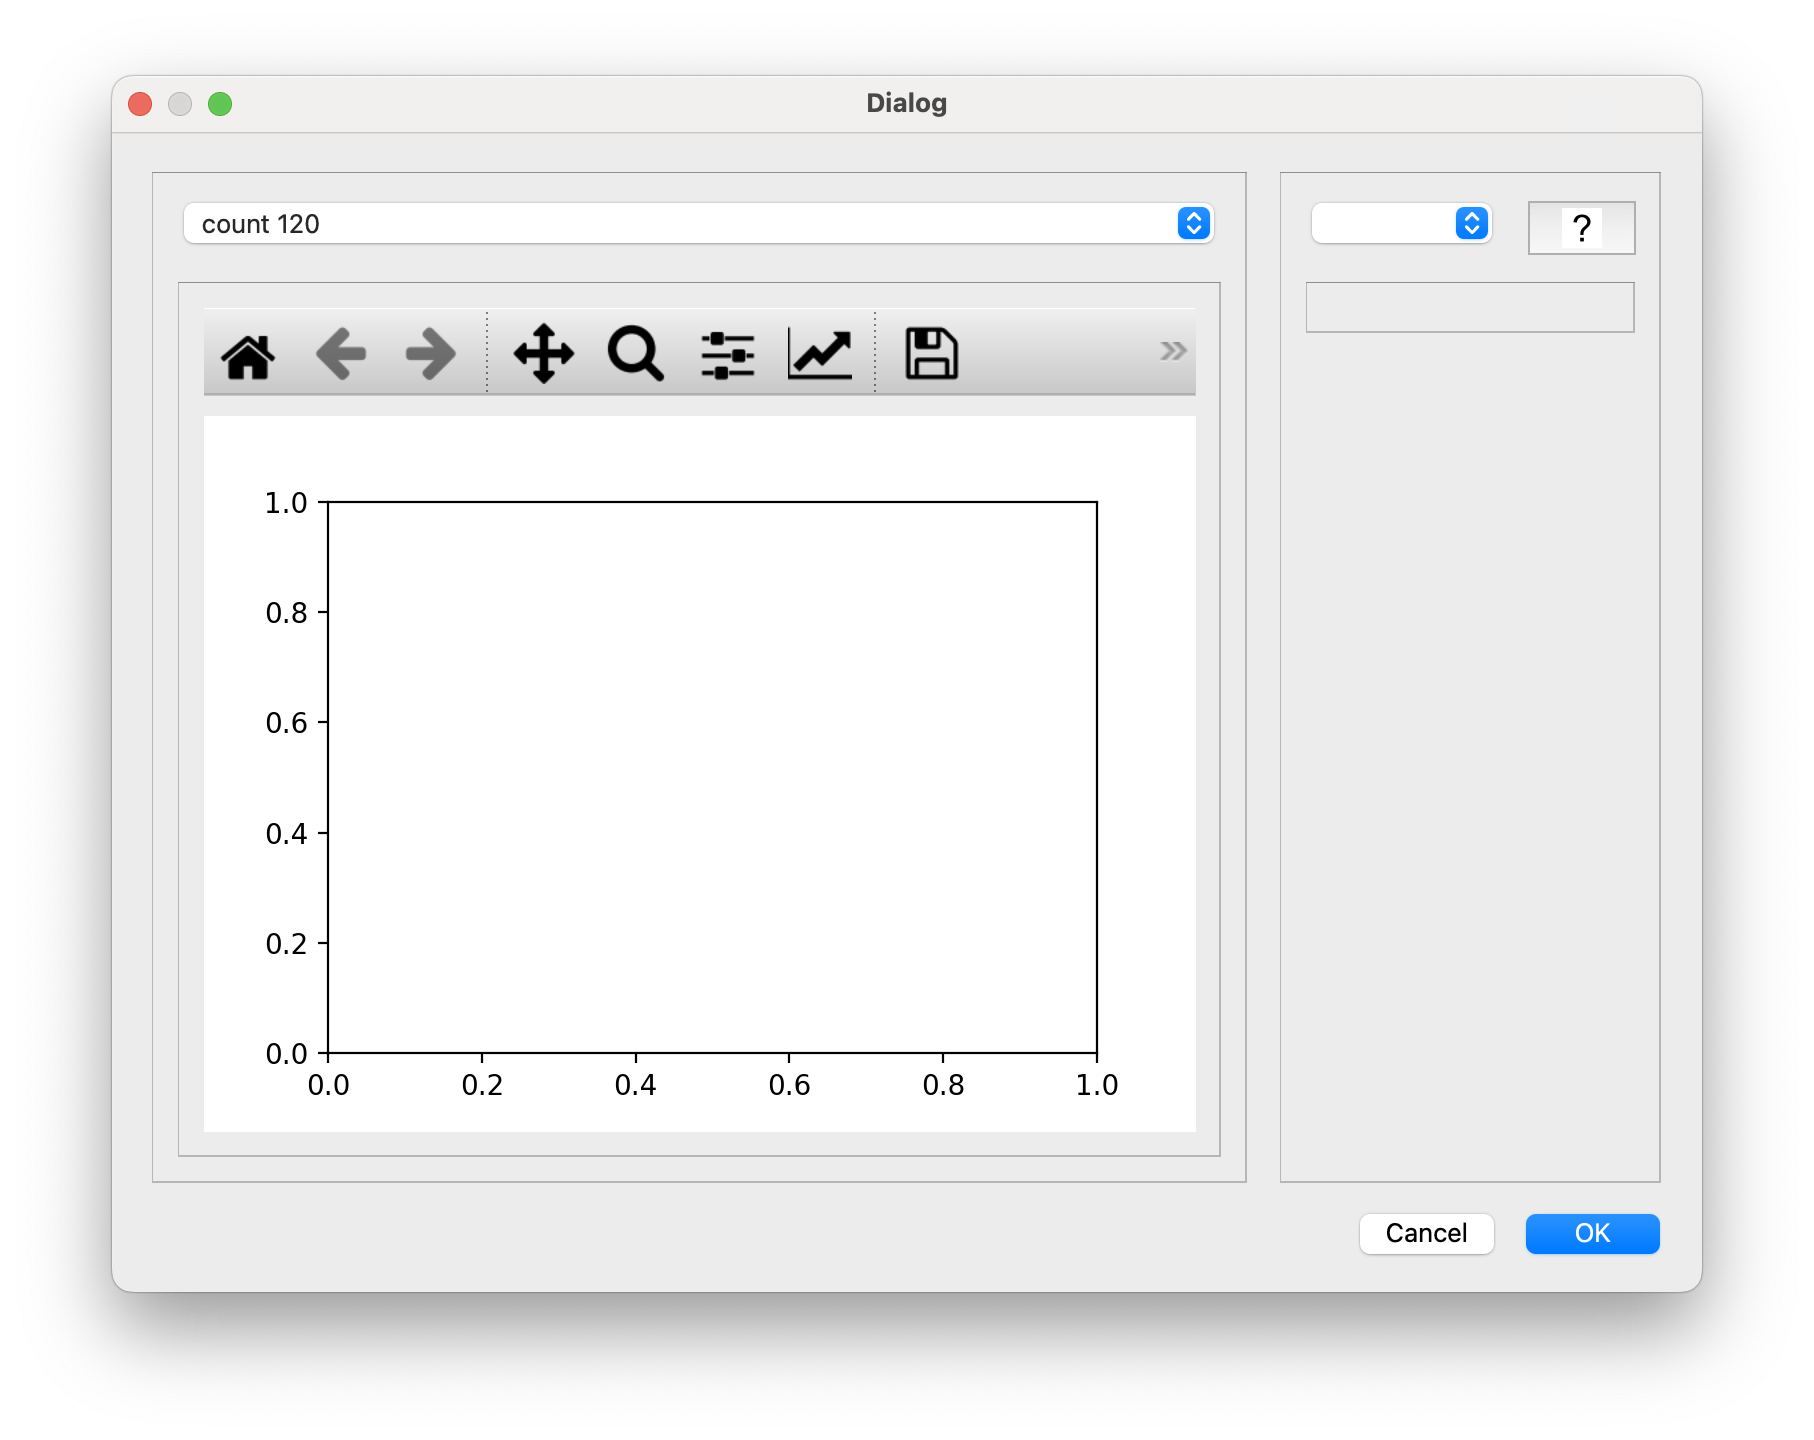
\includegraphics[width=\textwidth]{img/ParameterCurve.png}
        \end{center}
        \item We can now add functionailities to the GUI. First, we display the curve that we select in the combobobx. To do so, we will call the \texttt{handle\_data} function when the combobox is changed. This function will extract the data from the wrapper corresponding to the selected curve and plot it on the graph.
\begin{lstlisting}
def __init__(self, parent=None, wrp_base = None, path_base = None, path_curves = None, path_frequency = None, frequency = None):
    super().__init__(parent, wrp_base.get_child(path_base))

    if frequency is None:
        self.path_curves = path_curves
        self.path_frequency = path_frequency
        self.path_frequency_unique = None
    else:
        self.path_curves = None
        self.path_frequency = None
        self.path_frequency_unique = frequency

    # Initializes the graph
    self.cb_curves.currentIndexChanged.connect(self.handle_data)
\end{lstlisting}
        Note that we have also stored the paths to the frequencies associated to the curves in respectively the \texttt{path\_frequency} and \texttt{path\_curves} attributes. In the case where only one array is shown, then the path to the frequency array is stored in the \texttt{path\_frequency\_unique} attribute. 
        \item The \texttt{handle\_data} function extracts the path associated to a value in the combobox and gets both the Power Spectral Density and the frequency array from the wrapper corresponding to the selected curve. It then plots the data on the graph.
\begin{lstlisting}
def handle_data(self):
    """
    Plots the curve that is currently selected in the combobox. This function also defines self.data and updates the parameters.
    """
    # Extract the raw data from the wrapper corresponding to the selected curve in the combobox
    wrp = self.wrapper
    
    if len(self.combobox_curve_codes) > 1:
        path = self.combobox_curve_codes[self.combobox_curve_names.index(self.cb_curves.currentText())]
        path = path[5:]

        if type(path) == list:
            for e in path:
                wrp = wrp.data[e]
        else:
            wrp = wrp.data[path]
        
        self.data = wrp.data["Power Spectral Density"]
        if self.path_frequency is None:
            self.frequency = wrp.get_child(self.path_frequency_unique)[:]
        else:
            self.frequency = wrp.get_child(self.path_frequency[self.path_curves.index(path+"/Power Spectral Density")])[:]
        
        # Plot the data
        self.graph_canvas.axes.cla()

        self.graph_canvas.axes.plot(self.frequency, self.data)
        self.graph_canvas.axes.set_xlabel("Frequency Shift (GHz)")
        self.graph_canvas.axes.set_ylabel("Intensity (AU)")
        self.graph_canvas.draw()
        self.update_parameters()
\end{lstlisting}
        Note that the last line of this function is calling the function \texttt{update\_parameters}. This function will update the list of parameters needed to run the treatment. 
        \item We can define the \texttt{update\_parameters} function. This function will most likely be common to most treatments. Its goal is to inspect the "treat" module from the \texttt{HDF5\_BLS} package and extract the list of functions and parameters that are needed automatically. Then it displays the list of functions in the dedicated combobox and the list of parameters in the dedicated frame. If the nomenclature of the parameters and the definition of the treatment function follow a fixed nomenclature, this function automatically links the graph with the relevant parameters so that the graph becomes interactive. Further information about how to develop new treatment functions can be found in section \hyperref[subsec:treatment.new]{Adding a new treatment function}. Out of curiosity, here is the detail of the code of this function:
\begin{lstlisting}
def update_parameters(self):
    def initialize_parameters(self, module):
        functions = [func for func in getmembers(module, isfunction)]
        function_names = [func[0] for func in functions]
        functions = [func[1] for func in functions]

        self.cb_functions.clear()
        self.cb_functions.addItems(function_names)
        self.cb_functions.setCurrentIndex(0)
        self.cb_functions.currentIndexChanged.connect(lambda: self.show_parameters_function(functions, function_names))

        return functions, function_names

    def setup_button_help_function(self, functions, function_names):
        def show_help_function():
            docstring = functions[function_names.index(self.function_name)].__doc__ or ""
            msgBox = HelpFunction(self, self.function_name, docstring)
            msgBox.exec_()

        self.b_helpFunction.clicked.connect(show_help_function)

    def onclick_x0(event = None):
        if event.inaxes:
            x = float(event.xdata) * 1e6//1
            x = x/1e6
            self.parameters["center_frequency"]["line_edit"].setText(str(x))
    
    def onclick_linewidth(event = None):
        if event.inaxes:
            self.temp_linewidth = float(event.xdata)
            self.graph_canvas.mpl_connect('motion_notify_event', on_drag)

    def on_drag(event):
        if event.inaxes and event.button == 1:
            x1 = float(event.xdata)
        linewidth = abs(x1 - self.temp_linewidth) * 1e6//1
        linewidth = linewidth/1e6
        self.parameters["linewidth"]["line_edit"].setText(str(linewidth))

    # Define the module to be used 
    import HDF5_BLS.treat as module 

    # Extracts the functions and the function names from the module
    self.functions, self.function_names = initialize_parameters(self, module)

    # Sets the combobox with the functions
    self.show_parameters_function(self.functions, self.function_names)

    # Adds the models in the dedicated combobox.
    Models = module.Models()
    self.parameters["c_model"]["combobox"].addItems(Models.models.keys())

    # Connects the QLineEdit widget to the onclick_x0 function
    self.parameters["center_frequency"]["line_edit"].mousePressEvent = lambda event: self.graph_canvas.mpl_connect('button_press_event', onclick_x0)
    
    # Connects the QLineEdit widget to the onclick_linewidth function
    self.parameters["linewidth"]["line_edit"].mousePressEvent = lambda event: self.graph_canvas.mpl_connect('button_press_event', onclick_linewidth)

    # Sets the help button to display the function's docstring
    setup_button_help_function(self, self.functions, self.function_names)
\end{lstlisting}
        Note that the last line of this function is calling the function \texttt{button\_help\_function}. This function is meant to display the docstring of the function in a dedicated window when the "Help" button is pressed on the interface.
        \item The next step is to allow the user to apply the selected function with the parameters defined in the dedicated frame. To do so, we will setup a "Treat" button in the "setup\_apply\_button" function. 
\begin{lstlisting}
def setup_button_apply(self):
    """
    Creates the layout for the buttons to apply the function.
    """
    layout = qtw.QGridLayout(self.frame_confirmParam)

    button_treat = qtw.QPushButton()
    button_treat.setText("Treat")
    button_treat.clicked.connect(self.apply_function)

    layout.addWidget(button_treat, 0, 0, 1, 1)
\end{lstlisting}
        Note that the button is connected to the \texttt{apply\_function} function. This function returns the entered parameters of the treatement so that it can be performed.
        \item The \texttt{apply\_function} function is meant to read the parameters of the treatment and return an object that will allow the treatment on either one or multiple arrays. This function is developped as a switch between the different treatment functions that were defined in the dedicated combobox. Therefore its structure is the following:
\begin{lstlisting}
def apply_function(self):
    """
    Creates the layout for the buttons to apply the function.
    """
    func = self.functions[self.function_names.index(self.function_name)]

    if self.function_name == "unicorn":
        # Extract the parameters proper to the "unicorn" treatment
    elif self.function_name == "elf":
        # Extract the parameters proper to the "elf" treatment
\end{lstlisting}
        As a more concrete example, here is the code for the \texttt{fit\_model\_v0} treatment function:
\begin{lstlisting}
def apply_function(self):
    """
    Extracts the parameters from the GUI and pplies the treatment to the data.
    """
    func = self.functions[self.function_names.index(self.function_name)]

    if self.function_name == "fit_model_v0":
        # Extract the parameters of the function
        dic = {}
        try:
            dic["center_frequency"] = float(self.parameters["center_frequency"]["line_edit"].text())
            dic["linewidth"] = float(self.parameters["linewidth"]["line_edit"].text())
            dic["normalize"] = not bool(self.parameters["normalize"]["checkbox"].text())
            dic["c_model"] = str(self.parameters["c_model"]["combobox"].currentText())
            dic["fit_S_and_AS"] = not bool(self.parameters["fit_S_and_AS"]["checkbox"].checkState())
            dic["window_peak_find"] = float(self.parameters["window_peak_find"]["line_edit"].text()) 
            dic["window_peak_fit"] = float(self.parameters["window_peak_fit"]["line_edit"].text())
            dic["correct_elastic"] = not bool(self.parameters["correct_elastic"]["checkbox"].checkState())
            IR_wndw = self.parameters["IR_wndw"]["line_edit"].text()
            if IR_wndw == "None": 
                dic["IR_wndw"] = None
            else:
                dic["IR_wndw"] = IR_wndw.replace("(","").replace(")","").replace(" ","")
                dic["IR_wndw"] = tuple(map(float, dic["IR_wndw"].split(",")))

            self.parameter_return["Parameters"] = dic
            self.parameter_return["Function"] = func

            qtw.QMessageBox.information(self, "Treatment parameters stored", "The parameters for the treatment have been stored. You can now close the window to apply the treatment.")
        
        except:
            qtw.QMessageBox.warning(self, "Error while retrieving parameters", "An error happened while retrieving the parameters")
\end{lstlisting}
        Note that the parameters are stored in the "parameter\_return" dictionnary. This dictionnary is meant to be returned to the \texttt{treat\_ui} module, which will then apply the treatment to the data.


        \end{enumerate}
    
    


\end{document}
